% Preamble
\documentclass[a4paper, 12pt]{article}
\usepackage[margin=1in]{geometry} % Set margin
\usepackage{pdfpages} % Insert pdf pages
\usepackage{amssymb,amsmath,amsthm, amsfonts} % Math libraries

% Custom commands
\newcommand{\sub}[1]{\subsection{\underline{#1}}}
\newcommand{\subsub}[1]{\subsubsection{\underline{#1}}}
\newcommand{\?}{\stackrel{?}{=}}
\newcommand{\R}{\ensuremath{\mathbb{R}}}
\newcommand{\F}{\ensuremath{\mathbb{F}}}
\newcommand{\Onef}{\ensuremath{1_{\F}}}
\newcommand{\Zerof}{\ensuremath{0_{\F}}}
\newcommand{\eqbcuz}[1]{\text{~$\stackrel{(#1)}{=}$~}}
\newcommand{\eq}[1]{\begin{align*}#1\end{align*}}
\newcommand{\eqn}[1]{\begin{align}#1\end{align}}
\renewcommand{\qed}{$$\blacksquare$$}
\renewcommand{\b}[1]{\textbf{#1}}
\renewcommand{\because}[1]{~\b{(#1)}\\}
\renewcommand{\d}{\ensuremath{\Downarrow\\~}}
\newtheorem{lemma}{Lemma}

% Begin Document %
\begin{document}

% Title Page
\begin{titlepage}
    %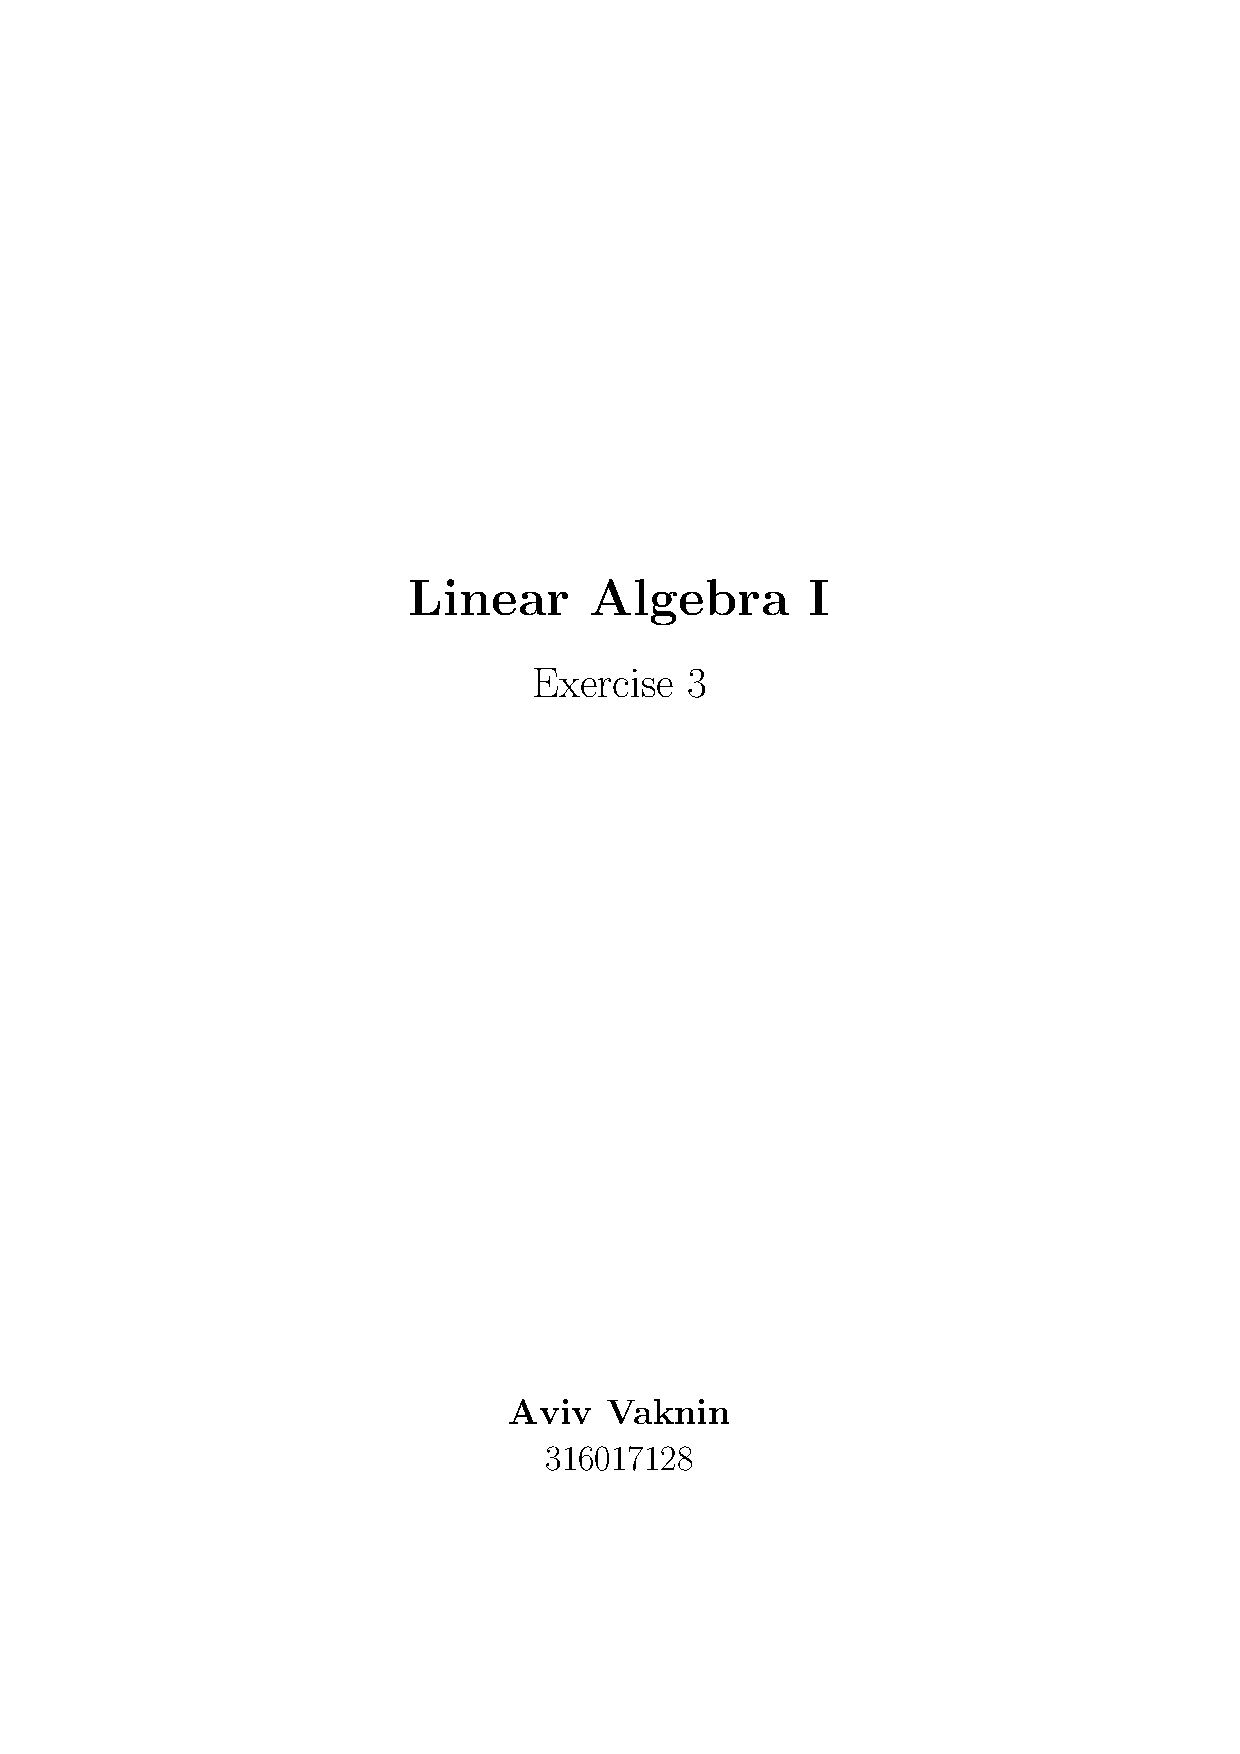
\includepdf{title.pdf}
\end{titlepage}

% 4
\setcounter{section}{3}
\section{Find the \textit{RREF} form for the given matrices:}
\sub{}
\eq{
    A=\begin{bmatrix}
        1&2&0&-1\\
        2&3&5&4\\
        4&8&13&12
    \end{bmatrix}
}
Working on the first column, we'll apply $A_2-2A_1$, and $A_3-4A_1$:
\eq{
    \begin{bmatrix}
        1&2&0&-1\\
        0&-1&5&6\\
        0&0&13&16
    \end{bmatrix}
}
For the second column, we'll apply $A_2\cdot(-1)$, and then $A_1-2A_2$:
\eq{
    \begin{bmatrix}
        1&0&10&11\\
        0&1&-5&-6\\
        0&0&13&16
    \end{bmatrix}
}
For the third column, we'll apply $A_3\cdot\frac{1}{13}$, $A_1-10A_3$ and $A_2+5A_3$, and therefore:
\eq{
    rref(A)=\begin{bmatrix}
        1&0&0&-\frac{17}{13}\\
        0&1&0&\frac{2}{13}\\
        0&0&1&\frac{16}{13}
    \end{bmatrix}
}
\sub{}
\eq{
    B=\begin{bmatrix}
        0&0&1&3&-2\\
        0&1&2&6&0\\
        0&2&3&8&2\\
        0&1&1&3&3
    \end{bmatrix}
}
We'll start with the second column, and replace $B_1$ with $B_2$.\\
Then we'll use $B_1$ to zero out the rest of the column, namely $B_3-2B_1$ and $B_4-B_1$:
\eq{\begin{bmatrix}
    0&1&2&6&0\\
    0&0&1&3&-2\\
    0&0&-1&-4&2\\
    0&0&-1&-3&3
\end{bmatrix}}
Now, for the third column, we'll apply $B_1-2B_2$, $B_3+B_2$ and $B_4+B_2$.
\eq{\begin{bmatrix}
    0&1&0&0&4\\
    0&0&1&3&-2\\
    0&0&0&-1&0\\
    0&0&0&0&1
\end{bmatrix}}
For the fourth column, we'll add $3B_3$ to $B2$, and then multiply $B_3$ by $(-1)$.
\eq{\begin{bmatrix}
    0&1&0&0&4\\
    0&0&1&0&-2\\
    0&0&0&1&0\\
    0&0&0&0&1
\end{bmatrix}}
For the last column, we'll apply $B_1-4B_4$ and $B_2+2B_4$, and therefore:
\eq{rref(B)=\begin{bmatrix}
    0&1&0&0&0\\
    0&0&1&0&0\\
    0&0&0&1&0\\
    0&0&0&0&1
\end{bmatrix}}
\sub{}
\eq{C=\begin{bmatrix}
    0&3&1\\
    5&-4&2\\
    2&2&7\\
    1&-1&0\\
    0&5&3
\end{bmatrix}}
We'll start with the first column, and replace $C_4$ with $C_1$, and then apply $C_2-5C_1$ and $C_3-2C_1$:
\eq{\begin{bmatrix}
    1&-1&0\\
    0&1&2\\
    0&0&0\\
    0&3&1\\
    0&5&3
\end{bmatrix}}
Now, for the second column, we'll apply $C_1+C_2$, $C4-3C_2$ and $C5-5C_2$:
\eq{\begin{bmatrix}
    1&0&2\\
    0&1&2\\
    0&0&0\\
    0&0&-5\\
    0&0&-7
\end{bmatrix}}
For the third and last column, we'll replace $C_3$ and $C_4$, multiply $C3$ by $-\frac{1}{5}$ and then apply $C_1-2C_3$, $C_2-2C_3$ and $C5+7C_3$, and get:
\eq{rref(C)=\begin{bmatrix}
    1&0&0\\
    0&1&0\\
    0&0&1\\
    0&0&0\\
    0&0&0
\end{bmatrix}}
\pagebreak

% 8
\setcounter{section}{7}
\section{Find all of the solutions, $\F=Q$}
First, let's convert the equations system into a matrix:
\eq{A=\begin{bmatrix}
    \frac{1}{3}&2&-6&|~0\\
    -4&0&5&|~0\\
    -3&6&-13&|~0\\
    -\frac{7}{3}&2&-\frac{8}{3}&|~0
\end{bmatrix}}
And then find its rref:
\eq{rref(A)=\begin{bmatrix}
    1&0&-\frac{5}{4}&|~0\\
    0&1&-\frac{67}{24}&|~0\\
    0&0&0&|~0\\
    0&0&0&|~0
\end{bmatrix}}
Therefore, we've received the following system:
\eq{\begin{Bmatrix}
    X_1-\frac{5}{4}X_3=0\\
    X_2-\frac{67}{24}x_3=0
\end{Bmatrix}}
We'll mark $x_3$ as $t_1$, therefore:
\eq{&x_1=\frac{5}{4}t_1\\&x_2=\frac{67}{24}t_1}
\eq{
    \mathbb{S}
    \begin{bmatrix}x_1\\x_2\\x_3\end{bmatrix}
    =
    \begin{Bmatrix}
        \begin{bmatrix}\frac{5}{4}t_1\\\frac{67}{24}t_1\\t_1\end{bmatrix}
    :
    t_1\in{Q}
    \end{Bmatrix}
}

% End Document %
\end{document}